%!TEX root = ../../thesis.tex
%!TEX enableSynctex = true
%*******************************************************************************
%****************************** Third Chapter **********************************
%*******************************************************************************
% **************************** Define Graphics Path **************************
\ifpdf
    \graphicspath{{Chapter/spt/Figs/Raster/}{Chapter/spt/Figs/PDF/}{Chapter/spt/Figs/}}
\else
    \graphicspath{{Chapter/spt/Figs/Vector/}{Chapter/spt/Figs/}}
\fi

\chapter{Diffraction limited single particle tracking in SPIM}

%Taken from Cat
\subsection{Introduction}
Herpesviruses are among the most complex and largest of the clinically relevant viruses.
Their virions possess a size of $\sim$ 200 nm and establish life-long infections in their hosts.
Herpesviruses are extremely widespread in vertebrates and humans.
For example, it is estimated that up to 85\% of the population worldwide are infected by herpes simplex virus 1 (HSV-1) and around 25% by HSV-2\.
Infections by the nine known human herpesviruses are associated with many serious diseases including certain lymphomas and life-threatening conditions in immuno-compromised patients \cite{[1]}.
Herpesviruses also cause a significant disease burden in animals that can lead to economic problems for livestock farmers.
Viral infections begin when infectious virus particles (virions) invade the organism by first attaching to and then entering susceptible cells.
After this initial event, viruses hijack the cellular machinery to replicate, produce progeny virus particles, and spread infection.
Herpesviruses pass through two distinct stages in their life cycle: lytic replication and latency.
Although many studies exist about the replication cycle of herpesviruses, not much is known about the later stages of the infection cycle, the assembly of virus particles and their egress from the cell.
Assembly and egress of viruses are essential stages in the herpesvirus lytic replication, hence contributing directly to pathogenesis.
Support for the today largely recognized model of assembly and egress was provided mostly by electron micrographs (reviewed in \cite{[2, 3]}).

\subsection{Herpesvirus structure}
The common virion morphology of herpesviruses suggests that also their mechanisms of assembly and maturation are comparable, although nucleotide or amino acid homology in genes and proteins between the three subfamilies is low due to a high degree of genetic and evolutionary diversity.
In herpesviruses, the DNA genome is packaged in a nucleocapsid which is enveloped by a lipid membrane containing many viral membrane proteins.
Nucleocapsid and envelope are separated by a complex, proteinacious matrix called the tegument.
Herpes simplex virus type 1 (HSV-1) is the most extensively studied herpesvirus, and is a general model for other alphaherpesviruses.
The capsid is built up by the capsid proteins (capsomers) and possesses an icosahedral symmetry (assembly of capsid reviewed in \cite{[4]}).
The tegument is a densely packed protein layer around the nucleocapsid, and essential for structural integrity and functionality of the virion.
While the nucleocapsid structure and protein composition is well understood, much less is known about the structure and assembly of the tegument.
The tegument can be divided into inner tegument (capsid-associated part) and outer tegument (envelope-proximal part).
The composition of the tegument varies for different herpesviruses.
For HSV-1, more than 20 viral tegument proteins are known \cite{[5, 6]}.
Most of these tegument proteins possess multiple functions e.g.
in the entry of viruses into the cell, transport of incoming nucleocapsids to the nuclear pore and genome release, as well as nuclear assembly and egress, nucleocapsid maturation and directed release from the cell.
Contained in the viral envelope of HSV-1 are at least 11 glycoproteins as well as several membrane-associated proteins which play important roles in viral entry and egress as well as virus-induced cell fusion \cite{[2, 7]}.


\subsection{Herpesvirus infection cycle}
To initiate infection, herpesviruses first bind to cellular surface proteins which act as virus receptors.
Due to direct fusion to the plasma membrane or endocytosis \cite{[8]}, the viral capsid is delivered into the cytosol.
Incoming capsids move towards the nuclear pore complexes by use of the cellular microtubule-associated motor system [9, 10].
There, they release the viral DNA through the nuclear pores into the nucleus \cite{[11]}.
Virion proteins drive the initial transcription to produce immediate early mRNAs.
Translation of these early mRNAs promotes further phases of viral gene transcription and replication of the viral DNA.
In ongoing, efficient infection, replication of viral DNA is provoked through actions of viral polymerases and other viral replicative machinery.
These replicated DNAs are used as templates for late mRNAs, which produce viral structural proteins, and are also packaged into capsids late in infection (reviewed in \cite{[4]}).
The egress pathway follows four steps (schematically shown in Figure 1):
(1) capsid assembly and genome encapsidation in the nucleus,
(2) primary envelopment and de-envelopment at the nuclear envelope,
(3) tegumentation and secondary envelopment in the cytoplasm, and
(4) exocytosis at the plasma membrane or cell-to-cells spread at cell junctions.
In the nucleus, capsid proteins autocatalytically coassemle with and around the so-called portal complex in late infection [4].
Nucleocapsid assembly is a very dynamic process.
The viral proteins have to recognize and cleave packaging signals at genomic termini, dock at the portal complex and pump the DNA inside the capsid [4].
After capsids are formed and packaged in the nucleus, the capsids have to traverse the nuclear envelope.
The nowadays largely accepted model proposes a process designated as nuclear egress.
The nuclear envelope consists of a double membrane - the inner and outer nuclear membranes (INM, ONM) - and therefore presents a strong physical barrier.
Mediated by several viral tegument and membrane proteins, the capsids bud into the INM (primary envelopment) to form an enveloped particle in the perinuclear space, fuse with the ONM (de-envelopment) and are released into the cytoplasm [12].
In the cytosol, capsids associate with more tegument proteins and bind onto and bud into cytoplasmic membranes derived from endosomes and/or the trans-Golgi network (secondary envelopment) \cite{[13, 14]}.
Although detailed mechanisms are not understood, it seems that tegument maturation is directly connected to secondary envelopment via direct protein-protein interactions.
Enveloped virions are secreted from cells by exocytosis [15, 16].

Figure 1: Scheme of assembly and egress pathway of virus particles.
From [2].
After capsids are formed in the nucleus, they bud into the inner nuclear membrane (INM) (primary envelopment) to form an enveloped particle in the perinuclear space.
These particles fuse with the outer nuclear membrane (ONM) (de-envelopment) and are released into the cytoplasm, leaving the envelope in the ONM.
In the cytosol, capsids bind onto and bud into cytoplasmic membranes (secondary envelopment), and enveloped virions are secreted from cells (release).
TGN, trans-Golgi network.
What is known about the early steps of tegument assembly?
Tegumentation occurs during virion maturation.
Complex protein-protein interactions mediate tegument assembly.
The intricate network of protein-protein interactions makes characterizing the precise function(s) of any individual protein difficult.
The tegument composition changes during assembly and egress (reviewed in [2, 17]).
The diversity of the tegument components raises the challenging question of how and where they are selected for incorporation into nascent virions.
Overall, it is supposed that early coating with few tegument proteins occurs at the nuclear stage, some viral proteins are shed during nuclear egress, and other tegument proteins are acquired in the cytosol and during secondary envelopment [18].
One would suspect that early tegumentation plays a role primarily for virus egress, i.e.
for directed transportation to the inner nuclear membrane, primary envelopment, de-envelopment and/or further unknown functions.
A recent study, using 3D single particle tracking, has shown that nuclear herpesvirus capsids do not use directed motility to reach the nuclear envelope.
Thus, viral proteins work by changing the nuclear architecture to create space for capsid free diffusion rather than activating capsids for transport [19].
After reaching the INM, budding occurs in order to transfer the capsids from the nucleus in the perinuclear space.
The viral proteins pUL31 and pUL34 form the so-called nuclear egress complex [20, 21], whose formation is crucial for budding [17, 22].
pUL34 is a membrane protein attached to nuclear membranes, and upon complex formation also pUL31 accumulates at the nuclear rim [20].
Both proteins are present on perinuclear capsids, but are then shed from the capsids and not existent on mature extracellular virions [17].
Contradicting results were published if and which proteins of the mature tegument assemble at the capsids already within the nucleus.
pUL36, pUL37, pUL41, pUL47, pUL48, pUL49, pUS3, ICP0, ICP4 are part of the tegument layer in mature virions and have been reported to partially localize within the nucleus.
These findings have not been confirmed in other studies, and it is unclear whether these proteins associate with the nuclear capsids [5, 23\-32].
Much evidence for early recruitment onto the capsids is found for pUS3, pUL36, pUL37, pUL41 and pUL49 which were identified in mature and perinuclear virions [18, 21, 33\-35].
An increasing volume of evidence suggests that ICP0 and ICP4 are present on mature virions, but the intracellular compartment where this interaction occurs is open for debate [35\-39].
Although they are not essential for nuclear egress [2], some of the putative early tegument proteins play a role in primary envelopment and/or de-envelopment [17, 40].
Finally, whether any other tegument proteins also interact with nuclear capsids is presently unknown.

\subsection{Single virus tracking}
While optical imaging is generally limited to a resolution of $\sim$ 250 nm by the laws of diffraction, sparse emitters can be localized with much higher precision by fitting a model function to their intensity distribution.
Beneath the methods of super-resolution imaging, awarded by the Nobel Prize in chemistry in 2014, the principles of localisation microscopy are also applied in single particle tracking (SPT) as was shown already in early single molecule studies [41, 42].
SPT is a real-time imaging technique that monitors the movement of individual particles and can provide information about dynamic behaviour in a cellular context.
Many studies exist on virus trafficking between and inside cells using single particle tracking (reviewed in [43]).
In general, more studies about the early stage of infection, virus entry and transport, exist than studies about the late stages of infection, virus assembly and egress.
Only few and recent works probe exclusively the molecular egress pathway of herpesviruses.
Hogue et al.
used total internal reflection fluorescence (TIRF) microscopy to selectively visualize fluorescent pseudorabies viruses near the plasma membrane and follow them during exocytosis [16].
Sandbaumhüter et al. could show by a motility analysis of fluorescent HSV-1 that directed transport of cytosolic capsids was dependent on both tegument proteins pUL36 and pUL37 [44].
The mentioned examples show that single-virus tracking can reveal detailed information about the dynamics of single viruses inside cells with high spatial and temporal resolution.
But due to a limited depth of field, particles observed in a 3D volume usually leave the axial detection range rapidly.
Thus, data analysis often relies on two dimensional projections of short trajectory fragments and might not accurately represent three-dimensional (3D) particle motion if the specimen structure is not isotropic [45].
Several technical approaches already exist to perform SPT in three dimensions [46-49].
In the field of virology, very few studies make use of 3D SPT to date.
Orbital tracking in two planes was applied to track prototype foamy virus (PFV) in real-time inside cells [50], and a rotating, oblique light sheet and astigmatic detection were used to image and track viral capsids with high temporal and spatial resolution inside the cell nucleus [19].
The new technical development opens up exiting perspectives in studying herpesvirus assembly and egress in vivo.


% \subsection{Aims}
% Until now, no quantitative and systematic approach exists that makes use of fluorescence microscopy with all its capacity in single molecule imaging to investigate herpesvirus tegument assembly inside infected cells.
% Generally, it is assumed that tegumentation starts directly after capsid formation, but direct evidence from live-cell data is missing.
% In the current project, we aim to prove that the first steps of tegumentation take place inside the nucleus.
% Several viral proteins have been identified as possible candidates for early tegumentation.
% We plan to investigate their cellular location, attachment to nuclear capsids and functional roles.
% In order to achieve our goals, we choose an interdisciplinary approach at the interface of advanced fluorescence microscopy, virus biology and quantitative single particle tracking.
% The methods we propose will allow us for the first time to look at both virion assembly state and motion through the cell at the same time.
% Bringing together the expertise of myself and my former group (Prof. Kubitscheck, single particle tracking) and the hosting institution (Prof. Kaminski, SPIM and superresolution imaging) in collaboration with Dr. Crump (virus biology) will make this an ideal combination for success.
%
% Which tegument proteins are assembled at the capsids in the nucleus?
% Several proteins of the mature tegument of HSV-1 have been suspected to assemble at capsids within the nucleus.
% We intend to investigate the presence of the following candidates inside the nucleus of infected cells and upon nuclear capsids:
% 1)	pUL36 and pUL37:
% pUL36 (>330 kDa) is most probably required for stabilisation of the capsid vertex-specific component (CVSC, a complex of capsid proteins pUL17 and pUL25) of nuclear and cytoplasmic capsids [51].
% The CVSC promotes nuclear egress of DNA-filled capsids by direct interaction of pUL25 with pUL31 [52].
% pUL36 mediates binding of pUL37, the second-largest tegument protein [53].
% Both proteins appear to link capsid and tegument [2].
% 2)	pUL47, pUL48, and pUL49:
% These are the most abundant tegument proteins in the mature virion, and act as central organizers of the tegument [54].
% pUL48 is recruited to capsids mainly by interaction with pUL36 [55].
% All three proteins are not directly involved in nuclear egress, but might help to organize and stabilize the early tegument.
% 3)	pUS3 and pUL13:
% Both proteins are kinases.
% pUS3 and pUL13 may participate in primary envelopment by regulating the localization of the HSV-1 pUL31/pUL34 complex at the inner nuclear membrane [21, 56-59].
% However, pUS3 itself is not essential for primary envelopment, but rather plays a role in de-envelopment [21, 56, 57].
% 4)	ICP0 and pUL41: The proteins are regulators of viral transcription, and host/viral translation and immune response, respectively [5].
% ICP0 is probably recruited onto the capsids by pUL49 [38].
% Incorporation of pUL41 may be facilitated by interaction with pUL48, pUL49 and possibly pUL47 [54].
% First, we will systematically image the cellular distribution of the mentioned tegument proteins, especially during the phase of capsid assembly and egress.
% Hence, we will use dual fluorescent viruses with capsid (pUL35 or pUL25) and tegument proteins of interest tagged with auto-fluorescent proteins (mTurquoise, EGFP and mCherry), and perform live-cell time-lapse imaging.
% In order to obtain image sequences with high quality and detail, we plan to apply a resolution- and contrast-enhancing imaging technique such as structured illumination microscopy (SIM).
% We will further investigate the attachment of the tegument to single capsids.
% We intend to analyze co-localization of capsid and tegument proteins using two approaches: (a) single particle tracking in combination with image correlation [60], and (b) correlation between dual-colour motion trajectories [61].
%
% What are the functional roles of early tegument proteins?
%
% Recently, it was discovered that nuclear capsids are not actively transported, but move mostly by free diffusion [19].
% Hence, we assume that the most probable functions of early tegument proteins consist in organization and promotion of nuclear egress and availability as binding partners for other tegument or viral membrane proteins.
% After screening which of the investigated proteins attach to capsids, we will determine the location of the tegumented capsids with regard to the nucleus structure.
% We assume that the location of attachment is connected to the functional role.
% E.g. pUL36 is supposed to stabilize the complex of the capsid-associated proteins pUL17 and pUL25, hence very early attachment of this protein near the sites of capsid assembly would be expected.
% pUS3, ICP0 and pUL13 have been described to be involved in primary envelopment, thus we would suspect that assembly of these proteins would occur near the nuclear membrane.
% In order to analyze if putative early tegument proteins play a role in primary envelopment, we will examine if binding of tegument proteins provokes changes in capsid mobility due to membrane interaction.
% Co-localization with the nuclear egress complex (labelled pUL31 or pUL34 proteins) will provide further evidence about participation in primary envelopment.
% In a final step, we will investigate in which order tegument proteins bind to capsids what will give evidence about in vivo protein-protein interactions.

\section{Single Particle Tracking}

%\section{Particle Tracking In Life Science}

%\subsection{Particle Tracking}

Particle tracking is a relatively young but vital tool in modern quantitative biology and the field of bio-informatics.
A particle can refer to anything that is particulate and is not exclusively large or small, circular or spherical etc.
These techniques are very useful at numerically quantifying and detecting large population movements to discern general trends.
For instance, pollen grain diffusion; a singular grain of pollen will be erratic and random whereas several hundred recorded paths will reveal a general diffusive trend through averaging.
Particle tracking lends itself very heavily to the study of intracellular dynamics, answering important biological questions such as: viral infection movement\cite{Brandenburg2007}, intracellular membrane dynamics\cite{Chenouard2014}, genome maintenance, gene transcript\cite{Planchon2011} and more\cite{Cognet2014}.

Particle tracking using light sheet microscopy is very relevant due to the high imaging speeds required to study particles that are both small and fast.
Confocal microscopes suffer because they cannot temporally resolve particles; widefield microscopes suffer because they cannot provide three dimensional data; SPIM can offer both.

\subsection{Particle spatial localisation}

Particle tracking can be broadly described as a two stage process, spatial localisation then temporal localisation.
%The spatial localisation of a particle involves accurately marking where one or many particles are within an image.
%Humans are naturally able to do this as they have evolved to notice patterns and anomalies.
%Programming a computer to undertake this exercise was an early feat in the field of computer vision\cite{Crocker1996}.
Crocker et al deconstructed the problem into logical computable steps.

Firstly Crocker's data was deconstructed as singular images in two dimensions rather than full video volumetric data.
Secondly each image was corrected for any distortion or error as digitised video is inherently imperfect and may not be truly representative.
Each image has a threshold found from an estimate of the background value of the image.
This threshold removes substantial noise that would otherwise contribute to the final result.
Pixels with local maximum brightness are identified as \emph{candidate} particles and compete with other candidates within a pre-defined radius slightly larger than the expected size of the particle.
\footnote{Methods since Crocker for a truly blind particle recognition have since been proposed but Crocker serves as a poignant historical but still relevant method of particle tracking using Computer Vision}

A centroid (centre of mass) fitting procedure is employed under the assumption that, to a first order approximation, spherical scattering emitters can be well-defined by a Gaussian profile.
By fitting a Gaussian profile and using tens of pixels to minimise error, particulate positioning can be defined to sub-pixel accuracy.
The most common method of Gaussian fitting due to its ease of implementation, speed, precision and robustness is iterative least squares fitting.

\paragraph{Overlap}

Crocker's method does not account for overlapping particle systems; experimental and computational methods are addressing this\cite{Serge2008}, but for the most part these cases are marked as rare outliers and typically rejected in particle tracking routines as samples are usually constructed with a sensible sparsity.


\subsection{Particle temporal localisation}

%The planet Pluto was originally discovered by Tombaugh in 1930 by comparing two images of the night sky a few hours apart.
%He would place an image in each side of his \textit{Blink comparator} and switch having his left or right eye open very quickly.
%With this he could intuitively notice trajectories of bodies in the sky.
%If his two images were taken years apart, his blink comparison metric would have been entirely chaotic.
%He chose a time span which ensured the that he could assign \textit{beyond reasonable doubt} likely trajectories between each image.

%The same principle applies to l
When localising particles temporally, images of particle distributions need to be taken swiftly enough so that any change in particle position is small enough such that it can be judged as the same particle but in a different position at a  time later, \textit{beyond reasonable doubt}.
Computationally this is achieved by assigning a global cost metric to the distance between particles which is then minimised to find the most likely solution of how particles in the first image have translated into the second image.

\subsection{Single Particle Tracking}

Tracking individual particles is an important tool for modern biology.
It has been used to study virus trafficking and how viruses penetrate the nucleus of a cell\cite{Brandenburg2007}; intracellular transport such as the movement of mRNA\cite{Spille2015a}; cell membrane dynamics\cite{Cognet2014} and more.


\subsubsection{Light sheet single particle tracking}

A very novel and exclusive way of full three dimensional particle tracking using SPIM has been proposed.
By using a static lightsheet and an XYZ translator one can move a particle back into the FOV laterally if it drifts.
Once the particle is re-localised, the encoded position on the \(z\) aspect of the stage is then equal to the position of the axial position of the particle by virtue of the repositioning.
The \(x\) and \(y\) position are then derived using Crocker's centroid fitting from the resulting image accurately in post processing.

This method vastly improves the lateral resolution of the SPIM system as well.
Volumetric methods would limit the lateral resolution to half the beam waist, \(\sim 1 \mu m\), whereas this method is exclusively limited by the step size of the z translator (which can be very high resolution when using piezoelectric crystals) and one's ability to ensure the particle is precisely central within the excitation laser (which is then dependent on the particle size).
Spille demonstrated this technique very successfully on a single molecule of mRNA (\(50 nm\)\cite{Spille2015a}) moving on the membrane of a nucleus\cite{Spille2015a}.
SPIM's speed makes the technique very enticing as it is unrivalled for the purposes of particle tracking.
See Figure\ref{fig:SPIMSPT}.

This method could then be further improved using a tunable lens excitation, by tracking the position of the particle in \(x\) using the tunable lens and \(y\) by narrowing the trace of the scan mirror, the temporal and spatial resolution of single particle tracking could be vastly improved yet again.
Z position information could also be encoded into the image by virtue of light beam intensity.
By ensuring the particle is limited to half of the beam profile of the light sheet, then intensity of the particle would be proportional to a Gaussian curve z position.
This method could prove to be faster, more accurate and less perturbing on the sample as mechanical motion would be removed.

\begin{figure}
	\centering
	\begin{subfigure}[b]{0.35\linewidth}
		\centering
		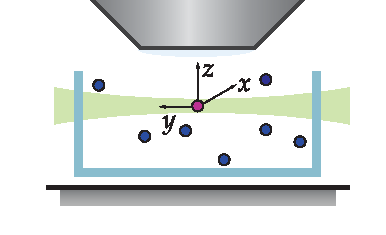
\includegraphics[width=0.8\linewidth]{Chapters/spt/Figs/PDF/tracking/1_piezo_track}
		\caption{Static Particle localised in \(xy\)}
		\label{fig:SPIMSPT1}
	\end{subfigure}
	\begin{subfigure}[b]{0.35\linewidth}
		\centering
		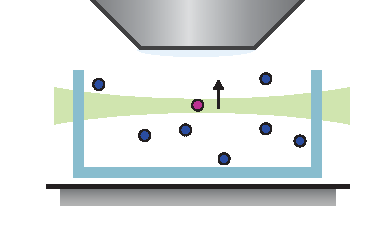
\includegraphics[width=0.8\linewidth]{Chapters/spt/Figs/PDF/tracking/2_piezo_track}
		\caption{Particle diffuses out of light sheet}
		\label{fig:SPIMSPT2}
	\end{subfigure}
	\begin{subfigure}[b]{0.35\linewidth}
		\centering
		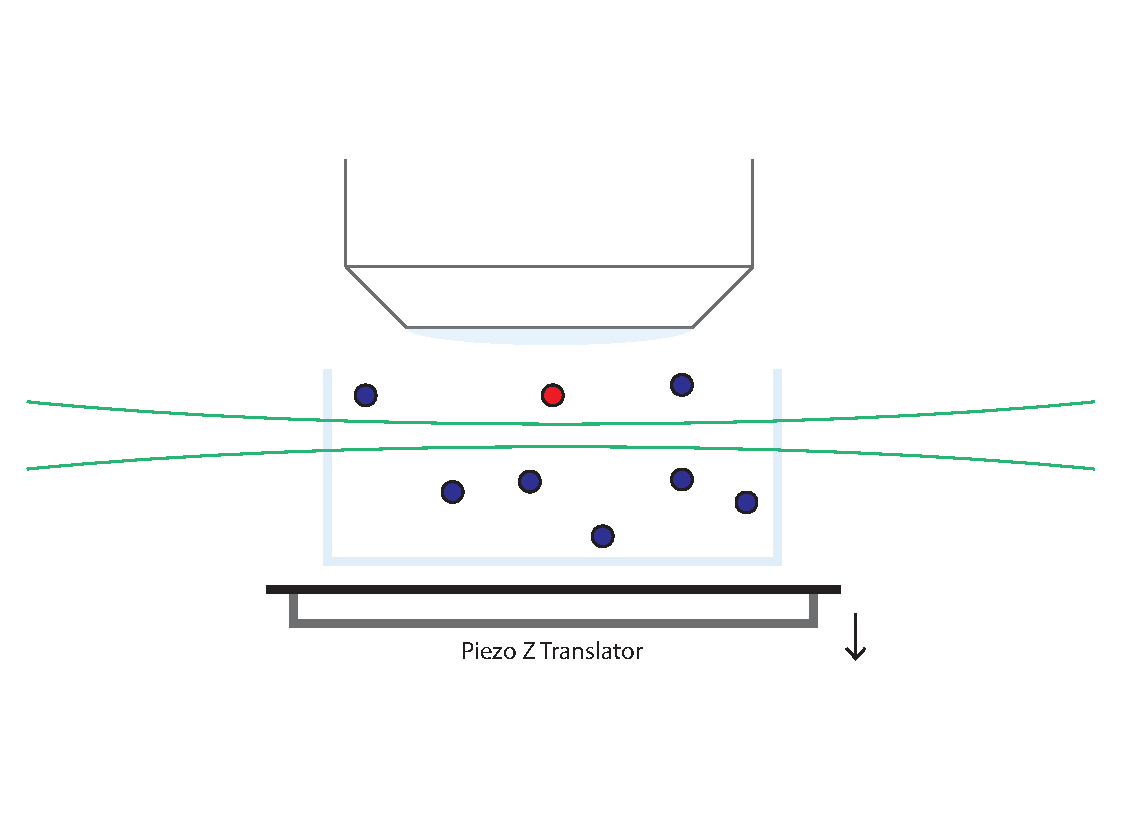
\includegraphics[width=0.8\linewidth]{Chapters/spt/Figs/PDF/tracking/3_piezo_track}
		\caption{\(z\) stage repositions so that particle is within light-sheet}
		\label{fig:SPIMSPT3}
	\end{subfigure}
	\begin{subfigure}[b]{0.35\linewidth}
		\centering
		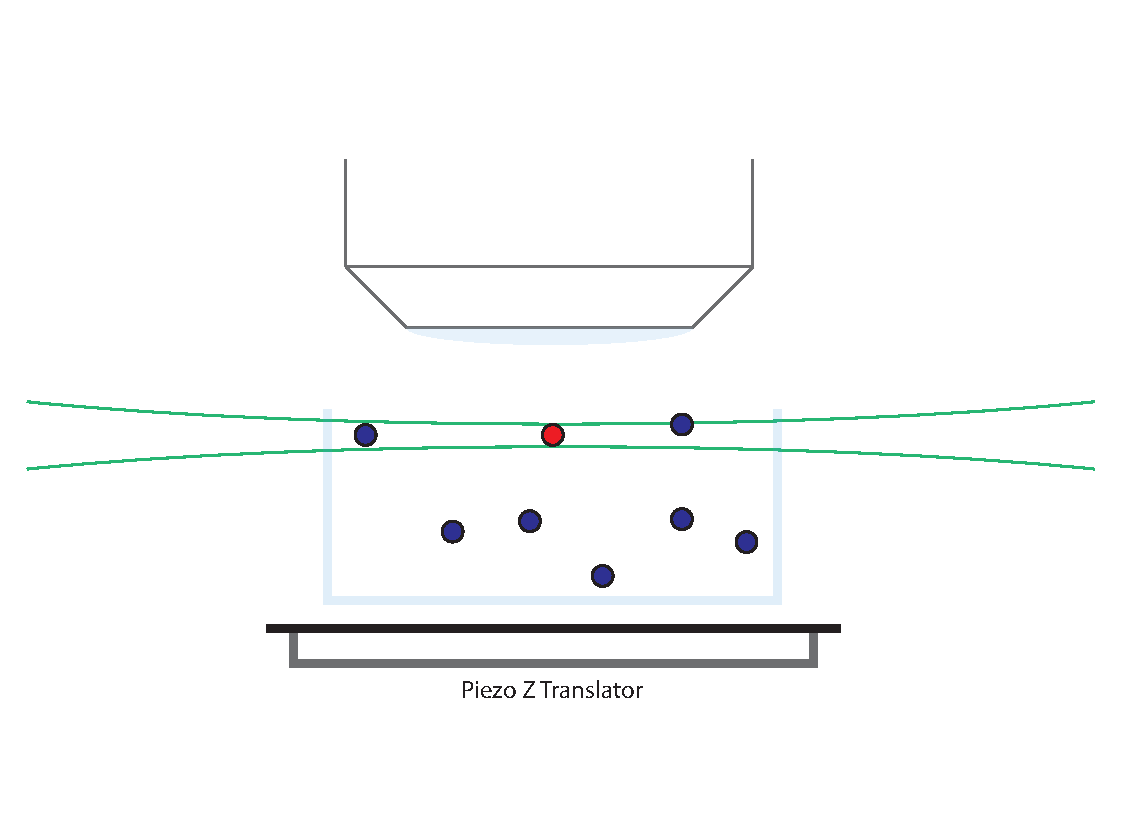
\includegraphics[width=0.8\linewidth]{Chapters/spt/Figs/PDF/tracking/4_piezo_track}
		\caption{Particle in light sheet, \(z\) position recorded}
		\label{fig:SPIMSPT4}
	\end{subfigure}
	\caption{Routine to track particles three dimensionally in SPIM}
	\label{fig:SPIMSPT}
\end{figure}

\subsubsection{Remote Focusing}

There are three ways in which to realise the full three dimensional SPIM.
The simplest way is to move the sample through the light sheet as is done in Oblique Plane Imaging.
The second method involves scanning the light sheet through \textit{z} which is potentially faster; the issue which then arises is that the light sheet moves out of the focal plane of the detection objective.
The focal plane can be moved onto the light sheet by moving the excitation objective, however this method (like the first method) causes perturbations to the sample.
Huisken \emph{et. al.} offer an alternative where the focal length of the objective is adjusted by placing a tuneable lens in the detection path (similar to section\ref{sec:tunable})\cite{Fahrbach2013}.
%Tunable lens technology is exceptionally young compared to the history of glass optics and so its image aberration correction is not as well implemented.
%To that end critics of this technique suggest that a tunable lens in the detection arm will inherently introduce noticeable image degradation.
Huisken showed that using a contrast grid that image quality and aberrations are negligibility affect and goes on to produce 100 Hz volumetric imaging though on small volumes\cite{Fahrbach2013}.

\section{Astigmatic Tracking}

To know whereabouts within the light-sheet the particle is so that the light-sheet may coarsely reposition, a finer axial localisation is needed across the waist of the sheet.
Adding a weakly cylindrical lens along the detection optics will add astigmatism to the point spread function of the microscope.
The asymmetry in focal lengths in the axes of the imaging plane means that in one axis the focal point will be offset axially compared to the orthogonal axis.
The result is that there in an overall axial asymmetry, and for point sources this allows axial position to be encoded in the image of the point source.
This technique was used to great effect in dSTORM and PALM systems which inherently rely on the localisation of point emitters.
The range over which an cylindrical lens can axial encode is at most \SI{\sim 1}{\micro\metre}, before the non-linearity in the astigmatism becomes too great and the PSF is too blurred to compute.

%Compare 2D guassian fitting ratio threatening
%\subsection{Fitting} %Guassian fitting
\subsection{Localisation}

Assuming a accurate localisation in 2D of a point emitter, the image of the astigmatic point emitter needs to then be compared to a calibrated sample.
This is achieved by holding a point emitter and precisely moving it axially and recording an image stack.
Typically the point emitter is held a gel-like phantom of the sample intending to be used.
Once the calibration volume has been recorded, a trade-off between speed and accuracy is made.

\subsubsection{Guassian fitting}
One of the slower techniques to recover axial position is fitting a 2D Gaussian.
The ratio of the FWHM of the Gaussian in the $x$ and $y$ directions will produce a calibration curve for axial position.
Attempting an iterative 2D Gaussian fitting in real-time is unrealistically with current computing capabilities, as such this technique is only useful in passive analysis of images already recorded.
%Talk about accuracy

\subsubsection{Template matching}


% Cros corelation
Cross correlation requires no fitting step and scales in computational complexity with the image as $O(n^2)$. %TODO check this
As such using as few pixels are feasible to recover axial position will allow this technique to function in real-time.
The cross correlation of two signals returns a single number representing an unnormalised similarity of the two signals.
Provided the astigmatism is transitioning linearly, a cross-correlation for every image in the calibrated stack may not be needed.
By using all the images in the calibration stack, the computational time increases by the half the number of axial images in that stack.
The ratio of the the cross correlation of two images spaced axially and equally about the focal centre of the stack will give an estimate of where the point is.
This estimate is sufficient for real-time results; and provided the images of the point-emitter are recorded, a more accurate axial localisation step can be applied in post-analysis.

\begin{align}
  I_{\text{Cross correlation}}
\end{align}

Similarly the covariance of the calibration an image or volume can be used, though the computational complexity is lower again.
%Talk about errors n shit
\begin{align}
  I_{\text{Cross correlation}}
\end{align}

\subsection{Simulations}

To verify that single particle tracking in light-sheet microscopy was possible, the diffusion of a single diffraction limited (infinitesimal point) particle was simulated \emph{in silico}.
To create the simulation, the particle was modelled to take a random walk of time steps $dt$ across a single imaging exposure of \SI{40}{\milli\second}.
This simulated how the particle would appear to move within the light-sheet.
The intensity of the final image of the particle was attenuated according to the Guassian intensity of the light-sheet axially($z$) and laterally ($x,y$) as per:

\begin{align}
  w_0 &= 1.4 \lambda \frac{ \text{NA}}{n}\\
  w(y) &= w_0 \sqrt{1+\left(\frac{y}{y_R}\right)^2}\\
  y_R &= \frac{\pi w_0^2}{\lambda}\\
  I(x,y,z) &= I_0 \left(\frac{w_0}{w(y)}\right)^2 e^{\left(-2\frac{z^2}{w(y)^2}\right)}
\end{align}

Where $w_0$ is the beam waist; NA is the numerical aperture of the excitation objective, $n$ is the refractive index of glass; $\lambda$ is the wavelength of excitation light; $y_R$ is the Rayleigh length and $w(y)$ is the beam waist through $y$.

\subsubsection{Astigmatism}

A false astigmatism was added to the simulation, to emulate an approximate response of the system.
To do this an Gaussian was convolved with the single point in space, with the assumption that the depth of field of the detection objective was longer than the width of the light-sheet.
To narrow Guassian as the particle moved through $z$ the standard Gaussian equation of:
\begin{align}
  f(x,y) = e^{-\frac{x^2 + y^2}{\sigma^2} }
\intertext{to}
  f(x,y,z) = e^{-\frac{x^2}{kz+c} +\frac{y^2}{-kz+c} }
\end{align}
Featuring an assumed linear astigmatism where $c$ is the bias value to create a minimum width of the particle the diffraction limited spot size and $k$ is the degree of astigmatism featuring.
In real optical systems astigmatism is non-linear but assumed to be linear for short distances from the focal plane.

\subsection{Assumptions}

It is assumed that a particle will not diffuse sufficently quickly as to cause a deviance to the PSF then used to characterise the location of the particle.
However, assuming the worst case of a particle diffusing in a straight trajectory (in the 2D case) the localised position of the particle will be the average of the start and end positions of the particle.
This smearing leads to very non-Guassian PSFs when diffusivity is high (Figure \ref{fig:})
Worse still, the PSF response of the particle is also axially depependet when using an astigmatic lens.
using the linear approximation of a linear astigmatic-like Guassian and assuming the worst case of a particle diffusing directly up, an analytical solution for the error incurred may be imputed:
\begin{align}
  {\int_{-\infty}^{\infty} \frac{\int_{0}^{L} e^{-\frac{x}{2(kz+c)}^2} dz}{e^{-\frac{x}{2kL+c}^2}} dx} \\
\end{align}
The above expression only considers $x$ and $z$ for simplicty of calculation.
The ratio of the linear Gaussian-like function and the expected ($e^{-\frac{x}{2kL+c}^2}$) Guassian is integrated over all space to provide an error value as a function of $L$ which is the distance the particle has traveled. %Which is related to the diffusion constant
The result of integrating over all space returns a function several infinities, so a smaller window is considered.
Using a factor of $c$ is valid as $c$ governs the minimal width of the PSF.

%insert solution.

\subsubsection{Analytical solution}

From the assumption of a near linear astigmatic response of the particle in the light-sheet, and ignoring the reduction in ene

\begin{figure}
  \centering
  %\includegraphics{/path/to/figure}
  \caption{A single diffusing in medium was simulated using near native cellular conditions to establish the viability of particle tracking in the microscope.}
  \label{}
\end{figure}

\subsubsection{PSF Smearing}

%Idealsied particle looks like
% Actual particle will have a smearing effect so you will always assume you've got less far in xyz
% When considers

\section{Results}

\subsection{Cellular imaging}
\subsubsection{Mounting}
%As seen in chapter X mounting on flat glass is difficult.
%Cell culture requires a buffered medium, with most commercial solutions involving atmospheric control
HeLa cells were infected with
HeLa cells were mounted on clean \SI{25}{\milli\metre} $\times$ \SI{25}{\milli\metre} coverslips.
Trypsin was used to help lift cells in culture into solution and was left to act for \SI{3}{\minute}.
10\% Foetal Bovine Serum (FBS) was added to deactivate the Trypsin as it is a protease enzyme and will further degrade the cells.
Coverslips were submerged in the cellular solution and left to adhere and culture on the glass.
3\% paraformaldehyde was used to fix cells for the preliminary visualisation experiments.

\begin{figure}
  \centering
  %\includegraphics{/path/to/figure}
  \caption{Three-colour composite 3D image, as rendered in Imaris, of a pair of SHSY5Y cells.
          DESCRIBE COLOUR CHANNELS AND MEANING AND STUFF}
  \label{}
\end{figure}


\section{SPT using SPIM}

The secondary optical relay was set to 2x magnification to unsure the camera was Nyquist limited and that there were sufficient pixels available to observe astigmatism on a single particle.
The weakly cylindrical lens ($f = \SI{1}{\metre}$) was inserted in between the secondary relay and the camera unit at \SI{40}{\milli\metre} away from the apeture of the camera.
This was found emperically to be sufficiently astigmatic by eye.
Adding a cylindrical lens in an infinity space amplifies the effect and so a custom lens would have been needed.

For calibration of the axial particle tracking an agarose gel of beads was imaged with objective and the light-sheet stepped through small axial steps.
Moivng the stage would have better emulated how a particle would behave optically, however, the mechanical resolution and hysteresis of the stage made this infeasible.

\begin{figure}
  \centering
  %\includegraphics{/path/to/figure}
  \caption{Graph showing calibration between axial depth within the light-sheet and METRIC}
  \label{}
\end{figure}

\section{Conclusions}

%Would've been good to calibrate more than one colour?
% severe issues surrounding lots of spherical aberration

\subsection{Future work}

\subsubsection{Neural Networks} %Need to try training using this using convolutional neural networks
%Also possible to

So far the techniques presented for localising particles in an astigmatic system relies on a singular calibrated point emitter.
A population of point-emitters with known axial positions would help mitigate errors.
It is possible to align multiple calibration volumes and create an averaged or model calibration volume to work with; but this method relies heavily on the alignment step.
Training a neural network could be a more robust method.
Neural networks take multiple inputs and produce a single output based on a back propagation step which helps determine the weightings on the \emph{neurons} in the hidden layer or layers.
Convolutional neural networks work in a similar fashion except that the weightings are image convolution steps; by using convolution steps the overall size of the neural network needed reduces making image recognition possible.

By training a neural network on a given input segmented input image, with the known output of axial position,



%C ancer, \textit{in vivo studies} have "progress[ed] in monitoring neurodegenerative disease pathobiology"\cite{Hoffman2005}
%3D imaging in \textit{in vivo} is desirable and currently use complimentary techniques (microCT) to create 3D.
\subsubsection{Neuro-degenerative Disease}

%Tau proteins misfold to cause neurofibrillary tangles.
i
Current Alzheimer's disease models suggest that Amyloid beta fibrils elongate creating Amyloid plaques.
These plaques then pathologically cause an over production of tau in the first affected neuron.
This over production in the first neuron quickly produces toxic levels of tau which propagate into neighbouring neurons, causing a cascade neuronal degeneration\cite{King2002}.

Mechanisms for AD are not fully understood but tau protein misfolding is expected to play a role in the pathology\cite{LaFerla2008}.
Our group has shown that extracellular tau proteins cause the endogenous over-production of tau proteins\cite{Michel2014a}.
The group has begun to observe tau propagation in axons two dimensionally.
Observing the movement of tau proteins between neurons three dimensionally would perhaps reveal the mechanisms by which tau pathology neurodegeneration occurs, more specifically how extracellular tau proteins originated.
It is hypothesised that stress impact may be a cause of the secretion of tau proteins causing the degeneration of other neurons\cite{Gavett2011,Patterson2014a}.
An \textit{in vivo} study in a live animal model being impacted could verify this using light sheet particulate tracking.

It is possible that tau proteins move too quickly to be successfully tracked.
In our group Tau proteins have been monitored to move between neurons via axons at a rate of \SI{480}{\micro\meter} per 20 minutes or 0.4 um per second.
A standard confocal image exposure is on the order of 2 to 3 seconds, meaning a tau protein could displace during the image acquisition by \SI{1.2}{\micro\meter}.
This movement during exposure could lead to a tau protein appearing to be of the order microns, whereas in fact it is of the order tens of nanometres.
Light sheet technology can image \SI{300}{} times faster and so a propagating tau protein would only move \SI{4}{\nano\meter} during an acquisition, less than the size of the protein and so an acceptable error.
Most importantly, tau is of comparable size to mRNA which has already been successfully tracked within a live cell using light sheet SPT\cite{Spille2015a}.

% \subsection{Virus Trafficking}
%
% Virus particles are of the same length scale as mRNA and tau proteins and so can also be tracked using light sheet SPT.
% Viruses reproduce by exploiting cell structure.
% A virus particle will interact with the cell membrane either singularly or in a plaque to release the contents of the virus inside the cell.
% Proteins are released to suppress the immuno-response and enable suitable conditions for the viral genome move into the cell.
% Once inside, the virus moves to areas within the cytoplasm or nucleus and begins replication.
% Replicated virons then leave the cell and the cycle continues.
% Individual virus particles may follow a multitude of different paths or even fails completely during infection.
% By tracking viral infection at the single virus level observers can deconstruct the dynamics of virus-cell interactions.
%
% There are several challenges in tracking virus particles.
% Firstly, viruses are small, varying from 20 to 200 nm, sub-diffraction limit. %Their speed may also be a factor %todo.
% Virus labelling is also difficult due to its size and nature.
% Fluorescent probes are comparable to the size of the virus and so can hinder infectivity.
% Proximity of the fluorescent probes due to virus size can also cause self-quenching within the probes\cite{Seisenberger2001}.
% Furthermore less than 1 \% of virus particles successfully reach the replication stage.
% Some viruses for instance require large plaques to breech a cell membrane.
% Finally a live tissue study is desirable in modern biology\cite{Brandenburg2007} which is logistically challenging in terms of mounting and ample preparation.
%
% Light sheet particle tracking can produce sub-diffraction limit 100 Hz video, resolution sufficient to watch virus particles \textit{in vivo}.
% Due to the low photo-toxicity of light sheet, multiple virus particles could be tracked concurrently without damaging the cell compared to confocal techniques.
% Light sheet has been used successfully on live tissue, in live animal models\cite{Keller2008} and importantly light sheet SPT has been used in a live cell\cite{Spille2013}.
% Light sheet particle tracking is by virtue three dimensional and \textit{in vivo} allowing an unprecedented level of detail in a viral study using this technique\cite{Hoffman2005}.
%
